\documentclass[tikz,border=8pt]{standalone}
\usepackage{amsmath,amssymb}
\usetikzlibrary{arrows.meta,automata,positioning,quotes}
\begin{document}
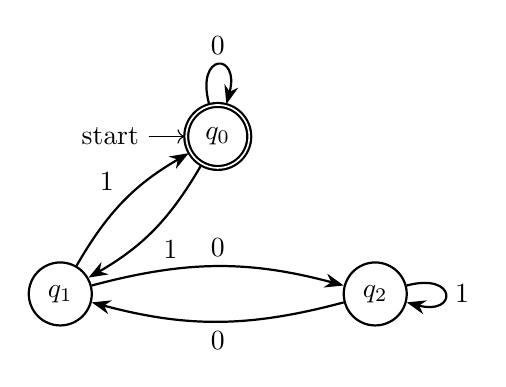
\begin{tikzpicture}[x=1cm,y=1cm]
\tikzset{
  graphnode/.style={circle,draw,thick,minimum size=8mm,inner sep=1pt,font=\sffamily},
  directed/.style={-{Stealth[length=2.4mm]},thick},
  undirected/.style={thick}
}
\node[graphnode,initial, accepting] (n_q0) at (0.00,2.00) {$q_0$};
\node[graphnode] (n_q1) at (-2.00,0.00) {$q_1$};
\node[graphnode] (n_q2) at (2.00,0.00) {$q_2$};
\draw[directed] (n_q0) to[loop above, "0"] (n_q0);
\draw[directed] (n_q0) to[bend left=15, "1"] (n_q1);
\draw[directed] (n_q1) to[bend left=15, "0"] (n_q2);
\draw[directed] (n_q1) to[bend left=15, "1"] (n_q0);
\draw[directed] (n_q2) to[bend left=15, "0"] (n_q1);
\draw[directed] (n_q2) to[loop right, "1"] (n_q2);
\end{tikzpicture}
\end{document}
